 % +++++++++++++++++++++++ remarque de DJOUADI Stationnement robotisé  supremi page 7
\chapter{Gestion du stationnement}
\markboth{Gestion du stationnement}{}
\section{Introduction}

La mise en œuvre d'une bonne gestion du stationnement est primordiale pour réduire les embouteillages, minimiser le temps de recherche de stationnement, favoriser la sécurité routière ainsi que contribuer à la création d’un environnement urbain plus fluide et confortable pour les citoyens.

Dans ce contexte, le premier chapitre explore le contexte générale de la gestion des parkings. Pour ce faire, nous avons commencé à définir le parking puis présenter les différents types de parking. Après cela, nous avons décrit les composants de base d’un système de gestion automatique de parking, ainsi que les meilleures pratiques en matière de gestion du parking. A la fin, nous avons effectué une étude de l’existant des zones de parking à Alger.


\section{Parking}
Étant donné que notre objectif est de réaliser un système de gestion du stationnement en temps réel, ce chapitre portera sur les bases du parking .

Le parking, également appelé parc de stationnement, est une zone spécialement conçue pour permettre aux véhicules de stationner, de manière temporaire ou prolongée. Il peut être public ou privé, situé en intérieur ou en extérieur. On peut trouver des parkings dans différents endroits tels que les aéroports, les hôpitaux, les bâtiments et les grands marchés, entre autres. Quant à la tarification, il peut être gratuit ou payant, selon les politiques de gestion mise en place \cite{parking}.\\
Le parking est souvent aménagé pour offrir une circulation fluide et sécurisée pour les véhicules. Il peut inclure également des services supplémentaires tels que la surveillance, le nettoyage de la voiture, le lavage et bien d'autres encore. Ces facilités visent à rendre le stationnement plus pratique et confortable pour les utilisateurs.
Son objectif est de répondre aux besoins de stationnement des conducteurs de véhicules dans les zones à forte densité de population et de trafic \cite{blog-direct-signaletique}.

une bonne gestion du parking contribue à une planification urbaine efficace, à la réduction de la congestion, à la promotion de la mobilité durable, à l'amélioration de la qualité de vie et à la gestion judicieuse des ressources financières.

\section{Types de parkings }

Les parkings peuvent être classés en plusieurs types en fonction de leurs caractéristiques (architecture du  parc, mode de paiement, accessibilité au parking, et la manière de stationnement) et de leurs utilisations \cite{evo-park}.

\subsection{Selon l'architecture  } 
Les parcs de stationnement les plus courants sont :
\begin{outline}
\1 \textbf{ Parcs de stationnement en surface:} sont les parkings les plus simples, situés généralement au niveau du sol. Ils peuvent être revêtus d'asphalte ou de béton et ne possèdent pas de structures ni de toits. Vous les trouvez fréquemment dans les centres commerciaux, les écoles et d'autres lieux publics, comme illustré dans la figure ci-dessous \ref{Surfacepark}.

\begin{figure}[H]
	\centering
	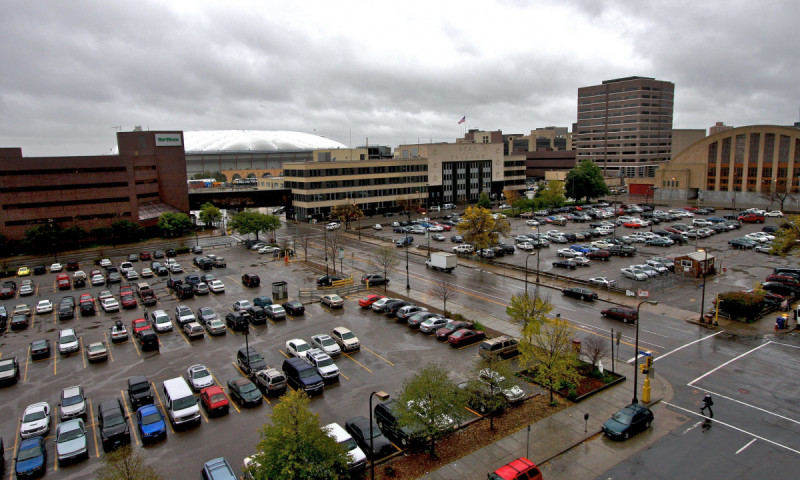
\includegraphics[height=05cm]{img/ch1-Surface parking-01.jpg}
	\caption{Parc de stationnement en surface}
 \label{Surfacepark}
\end{figure}

\1 \textbf{ Parcs de stationnement à étages: } Les parcs de stationnement à étages sont des structures qui ont plusieurs niveaux pour garer les voitures. Ils sont souvent faits de béton ou d'acier et ont des rampes ou des ascenseurs pour monter ou descendre entre les niveaux. Ces parkings peuvent être gérés automatiquement ou manuellement, et ils peuvent être couverts ou en plein air. Vous les trouvez souvent en ville, comme le montre l'image ci-dessous.. \ref{storeypark}.

\begin{figure}[H]
	\centering
	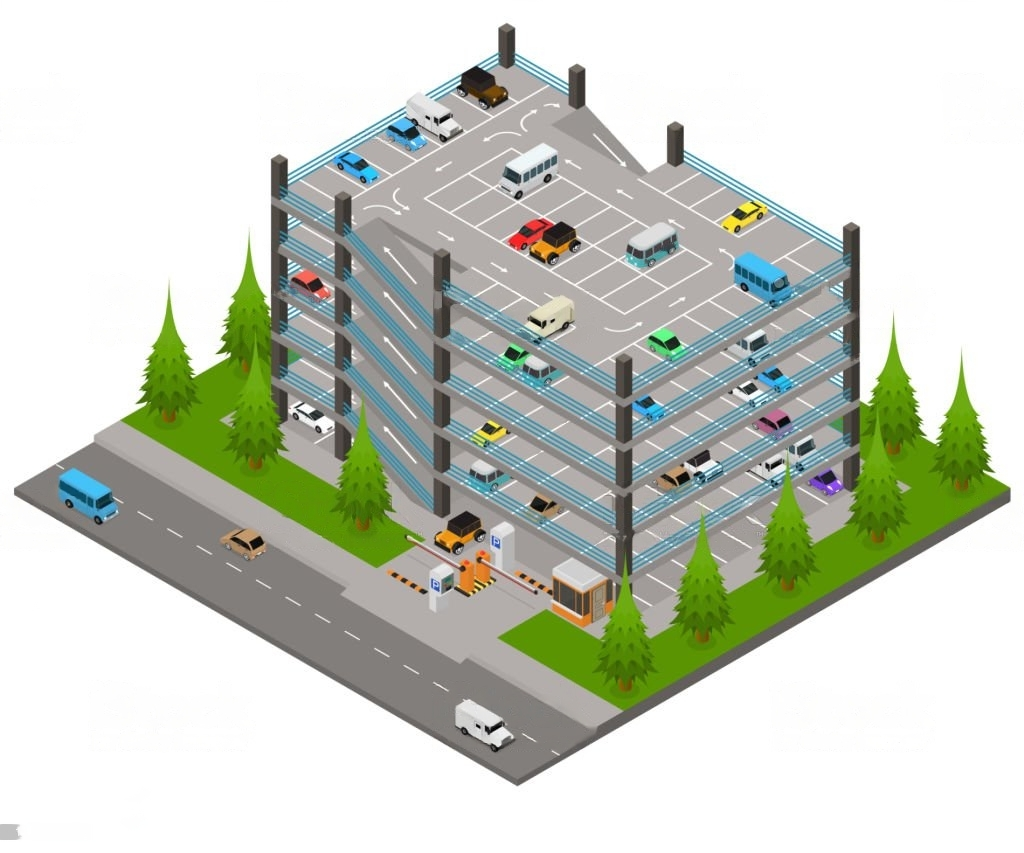
\includegraphics[height=06.5cm]{img/ch1-Multi-storey parking garages-01.jpeg}
	\caption{Parc de stationnement à étages}
 \label{storeypark}
 \end{figure}


%\textcolor{red}{}
\1 \textbf{Parcs de stationnement souterrains: } il s'agit de structures de stationnement situées sous le niveau du sol. Ils sont généralement accessibles par des rampes ou des ascenseurs et sont souvent utilisés dans des zones fortement peuplées où l'espace est limité. Ces parkings sont souvent gérés par des opérateurs et peuvent être équipés de systèmes de sécurité et des systèmes d'aération avec de nombreuses ventilations \cite{yespark-lexique}. Ils peuvent être couverts ou en plein air selon les besoins et sont largement utilisés dans les zones urbaines où l'espace est précieux comme montre l'image suivante \ref{Undergroundpark}.

\begin{figure}[H]
	\centering
	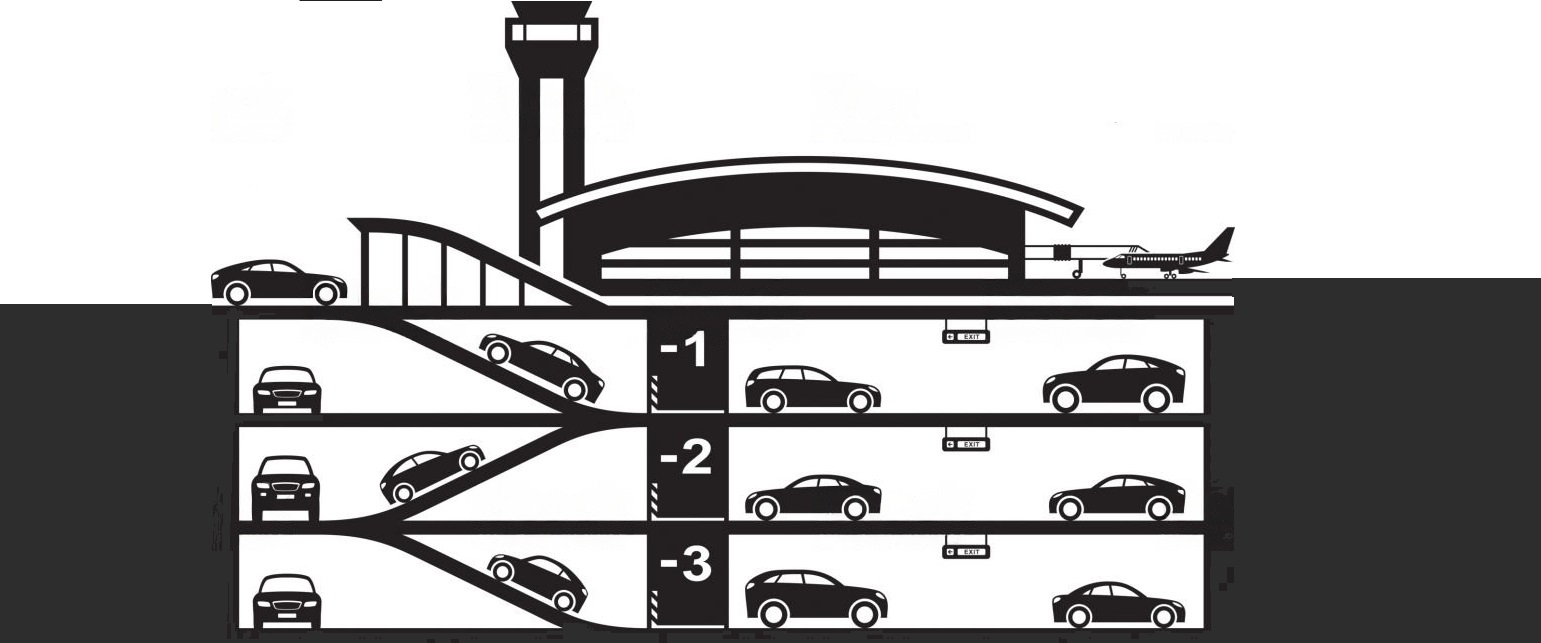
\includegraphics[height=06cm]{img/ch1-Underground parking garages-01.jpeg}
	\caption{Parc de stationnement souterrain}
 \label{Undergroundpark}
\end{figure}


\end{outline}

\subsection{Selon le mode de gestion}
Les types de parkings se différencient selon les modes de gestion en deux grands types, selon le paiement et la tarification, et selon l'accessibilité .

\subsubsection{Selon le mode de paiement}
Les parkings peuvent être classés en deux catégories principales, à savoir les parkings payants et les parkings gratuits.
\begin{outline}
    \1 \textbf{Stationnement payant par durée de stationnement/ illimité :} dans un parking payant, les utilisateurs doivent payer un montant prédéfinit ou un tarif forfaitaire  (quelle que soit la durée de stationnement) pour pouvoir se garer.
    \1 \textbf{Stationnement gratuit pour un temps limité/ illimité:}
    dans certains parkings gratuits, les utilisateurs peuvent stationner leur véhicule sans avoir à payer de frais pendant une durée limitée, généralement une ou deux heures. D'autres parkings gratuits offrent la possibilité de garer la voiture sans limite de temps. Ces parkings sont souvent situés dans des zones résidentielles ou des zones à faible trafic.
\end{outline}

Le choix entre un parking payant ou gratuit dépend souvent de la disponibilité, de la commodité, du coût et des préférences individuelles.

\subsubsection{Selon l'accessibilité}
On peut distinguer trois types de parkings en fonction de leur accessibilité : les parkings privés, les parkings publics et les parking privés à usage public \cite{lepermislibre}.

\begin{outline}
    \1  \textbf{Un parking public: } est un parking possédé et géré par des organismes publics, généralement la municipalité. Il est souvent situé en ville et hors agglomérations pour accueillir tous les usagers. Les parkings publics sont ouverts à tous, offrant ainsi une option de stationnement accessible à les usagers de la route.
    \1  \textbf{Un parking privé: } est un parking qui appartient et géré par des propriétaires privées ou des entreprises. Son accès peut être gratuit ou payant, et il peut être restreint par un badge ou une carte de stationnement. Les parkings privés sont généralement réservés aux clients, aux résidents ou aux employés d'un bâtiment spécifique, tel qu'un hôtel, un immeuble de bureaux ou un centre commercial. 
    \1  \textbf{Un parking privé à usage public: } est un parking appartenant à une entité privée qui est ouvert au public. 
    Un exemple courant de ce type de parking est celui des supermarchés. Ces parkings appartiennent au supermarché, mais ils sont accessibles à tous les clients qui souhaitent y circuler et s'y garer.

\end{outline}

Le choix entre un parking public et un parking privé dépend des circonstances individuelles, telles que l'emplacement, l'accès et les besoins spécifiques des conducteurs. 

% \subsection{Selon la méthode de stationnement}
% \begin{outline}
%     \1  \textbf{Stationnement conventionnel: } est la méthode traditionnelle de stationnement où les conducteurs trouvent et occupent manuellement une place de stationnement. Les conducteurs conduisent leur véhicule jusqu'à le parc de stationnement disponible et effectuent les manœuvres nécessaires pour s'y garer. Cette méthode de stationnement est largement répandue et utilisée dans les parkings conventionnels.
    
    % \1  \textbf{Stationnement robotisé (autonome): } il s'agit d'une méthode innovante où elle fait recours aux structures de stationnement automatisée (i.e systèmes robotiques) pour stationner et récupérer les véhicules sans intervention humaine. Dans ce type de système, les véhicules sont conduits jusqu'à une zone d'entrée spécifique où des capteurs et des logiciels avancés prennent le relais. Les véhicules sont guidés via les panneaux et signaux automatiques, puis déplacés automatiquement vers les emplacements de stationnement disponibles et les plus adaptés à leur taille à l'aide de mécanismes robotiques. Lorsque les conducteurs souhaitent récupérer leur véhicule, celui-ci est ramené à la zone de sortie par le système automatisé. Ce type de stationnement offre de nombreux avantages notamment l'utilisation optimisée de l'espace, une meilleure efficacité du stationnement et une réduction des risques de collision. l'illustration dans la figure  \ref{Automaticcarpark} 
    
% \begin{figure}[H]
% 	\centering
% 	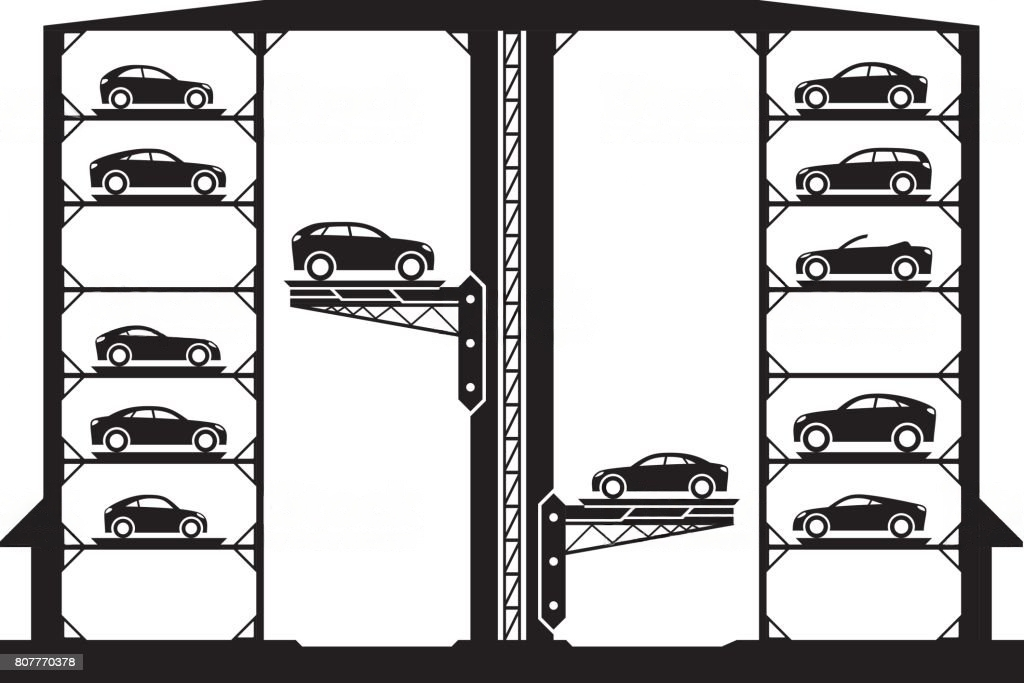
\includegraphics[height=06cm]{img/ch1-Automatic car parking -01.jpeg}
% 	\caption{Parc avec stationnement autonome}
%  \label{Automaticcarpark}
% \end{figure}



% \end{outline}

\section{Gestion des parkings}

La gestion des parkings peut varier en fonction du niveau d'automatisation impliqué \cite{bensalah-master}. On peut distinguer trois types principaux de gestion de parking :

\begin{outline}

\1  \textbf{Une gestion manuelle: } dans un parking à gestion manuelle, 
toutes les opérations sont effectuées par le personnel de service. Cela inclut l'accueil des conducteurs, la collecte des frais de stationnement, l'orientation vers les places disponibles et la surveillance générale du parking. 
Les employés sont responsables de toutes les tâches liées à la gestion du parking, au guidage des conducteurs et l'enregistrement de toutes les informations relatives aux parkings, que ce soit dans un registre ou dans un système informatique. Lors de leur arrivée au parking, les automobilistes reçoivent un ticket (en papier ou de bons d'entrée) et doivent le présenter au personnel de service lorsqu'ils quittent le parking pour régler les frais de stationnement. Ce type de système est généralement utilisé dans les petits parkings ou dans les zones où l'automatisation n'est pas encore largement répandue. Toutefois, il  présente une consommation importante de ressources et est sujet à de nombreuses erreurs et corruptions.


\1  \textbf{Une gestion semi-automatique: } dans un parking à gestion semi-automatique, certains aspects du processus de gestion sont automatisés pour améliorer l'efficacité. Par exemple, l'accueil des conducteurs et la collecte des frais de stationnement peuvent être effectués à l'aide de systèmes de paiement automatisés ou de bornes de paiement. De plus, des panneaux électroniques peuvent être utilisés pour indiquer les places disponibles. Ainsi que des barrières d'entrée et de sortie automatisées peuvent être utilisée pour contrôler l'accès des véhicules. Cependant, certaines tâches nécessitent toujours une intervention humaine, comme l'orientation des conducteurs vers les places de stationnement qui se fait par un agent de stationnement. Ce type de système offre une certaine automatisation tout en conservant une certaine interaction humaine.


\1 \textbf{Une gestion entièrement automatisée: } Dans un parking à  gestion automatisée, la majorité, voire toutes les opérations de gestion sont automatisées et aucune intervention humaine n'est nécessaire. 
Des systèmes informatisés ainsi que des technologies avancées sont utilisés pour effectuer toutes les opérations de gestion du stationnement notamment la collecte des frais de stationnement, l'orientation des conducteurs vers les places disponibles et la surveillance du parking. Ces systèmes offrent une gestion plus efficace et souvent utilisés dans les parkings à grande échelle ou dans les zones à forte densité de circulation.

\end{outline}
La méthode de gestion du stationnement à adopter dépend des besoins spécifiques de chaque emplacement et des ressources disponibles pour sa mise en œuvre.

\section{Systèmes de gestion des parkings}

Les systèmes de gestion des parkings sont des solutions technologiques utilisées pour optimiser l'efficacité et la gestion des parkings. Ils peuvent inclure une variété de fonctionnalités et d'outils pour faciliter la réservation, le contrôle d'accès, la collecte des frais de stationnement, la surveillance en temps réel, la gestion des données et la génération de rapports sur l’occupation du parking et la génération de revenus. 

Les parkings dotés de systèmes de gestion intègrent généralement les fonctionnalités suivantes:

\begin{enumerate}
   \item [$\bullet$]  Guidage des véhicules: Les parcs de stationnement automatisés sont équipés de systèmes de guidage qui aident les conducteurs à trouver rapidement des places de stationnement disponibles. Cela peut inclure des panneaux indicateurs, des feux de signalisation et des indications visuelles pour diriger les conducteurs vers les emplacements libres.
    \item [$\bullet$]  Contrôle d'accès automatisé : Les parcs de stationnement automatisés utilisent des systèmes de contrôle d'accès automatisés pour gérer l'entrée et la sortie des véhicules. Cela peut se faire à l'aide de cartes magnétiques, de codes QR, de lecteurs de plaques d'immatriculation ou d'autres technologies d'identification et de reconnaissance.
     \item [$\bullet$] Comptage de véhicules : Pour connaître l'état du parking, des capteurs en temps-réel sont utilisés pour compter le nombre de véhicules présents dans le parking, le nombre de places occupées/vacantes, fournissant des données précieuses pour la gestion et la planification.
   \item [$\bullet$] Empilement automatique des véhicules : Dans des parcs à espace limité, les véhicules sont empilés et stockés de manière automatisée grâce à des systèmes mécanisés d'empilement. Cela permet d'optimiser l'utilisation de l'espace en réduisant l'encombrement et en permettant le stationnement de plus de véhicules dans une superficie limitée.
    \item [$\bullet$] Surveillance temps-réel et sécurité renforcée : Les parcs de stationnement automatisés sont équipés de mesures de sécurité avancées, telles que des caméras de surveillance, des systèmes d'alarme et des dispositifs de sécurité pour assurer la protection des véhicules et des utilisateurs.
    \item [$\bullet$] Paiement automatisé : Pour permettre 
   aux utilisateurs de régler facilement les frais de stationnement, les parcs peuvent être équipés des bornes de paiement automatisée.
   Ces bornes peuvent accepter différents modes de paiement, tels que 
   le paiement sans contact ou paiement mobile.
   \item [$\bullet$] Gestion des abonnements : Permettant aux abonnés d'accéder facilement au parking en utilisant des cartes bancaires, ou des badges d'abonnement, en offrant donc  un accès rapide et pratique aux abonnées.
  \item [$\bullet$] Gestion de réservation: Permettant aux utilisateurs de réserver à l'avance une place de stationnement dans le parking, garantissant ainsi leur disponibilité lors de leur arrivée. Elle est effectuée en ligne, généralement via un site Web ou une application mobile dédiée.
   \item [$\bullet$] Génération de rapports d'activité : Est une fonctionnalité essentielle. Les rapports d'activité fournissent des informations détaillées sur divers aspects du fonctionnement du parking telles que le nombre de véhicules entrants et sortants, la durée de stationnement moyenne, l'occupation du parking en temps réel, les revenus générés, les tendances de fréquentation, les heures de pointe, etc. Les données collectées par les différents outils du système, tels que les capteurs de stationnement, les dispositifs de paiement et les caméras de surveillance, sont centralisées et analysées pour produire des rapports pertinents. Les rapports peuvent être consultés à tout moment par les gestionnaires du parking, ce qui leur permet de suivre les performances du parking, de prendre des décisions éclairées basées sur des données concrètes et d'optimiser les opérations.

\end{enumerate}

En plus de ces fonctionnalités, d'autres technologies peuvent être intégrés, telles que les applications mobiles qui offrent aux utilisateurs des fonctionnalités pratiques telles que la recherche de places, la réservation, le paiement et la navigation vers le parking.

Le contrôle de l'ensemble du processus de stationnement se fait d'une manière centralisé via un système informatisé ou un logiciel de gestion du stationnement qui regroupe toutes les fonctionnalités nécessaires et assure une coordination efficace de l'ensemble du processus de stationnement. 
La sélection et la mise en place d'un système de gestion des parkings dépendent des besoins spécifiques de chaque site, de sa taille, de son type d'utilisation et des ressources disponibles. 

L'objectif de tels systèmes est d'améliorer l'expérience des utilisateurs (i.e expérience plus pratique), d'optimiser l'utilisation de l'espace de stationnement et des ressources disponibles, de réduire la congestion, d'augmenter la sécurité et d'optimiser la gestion des revenus.

Il est donc courant d'utiliser une combinaison d'outils pour créer un système de gestion du stationnement complet et efficace. 


\section{Outils utilisés dans un système de gestion du stationnement}
Dans un parking, les outils et les personnes ont des fonctions différentes mais complémentaires.

Dans le cadre d'un système de gestion automatique du stationnement, différents outils sont utilisés pour optimiser la gestion des parkings et des véhicules. Bien que le rôle du personnel travaillant dans le parking soit généralement réduit par rapport à un système traditionnel, leur présence demeure importante pour offrir une assistance en cas de problèmes ou des situations imprévues. Leur présence garantit une expérience client optimale et contribue à assurer le bon fonctionnement global du système de gestion automatique du stationnement.

Parmi les outils basiques utilisés, on retrouve les barrières et les portes tournantes qui sont utilisées pour contrôler l'accès des véhicules au parking, ainsi que les portillons sont employés pour restreindre l'accès des piétons à certaines zones. Les caméras de surveillance et les systèmes d'interphone aident également à améliorer la sécurité et la surveillance, permettant aux opérateurs de surveiller les activités dans le parking. De plus, les panneaux de signalisation sont installés pour informer les conducteurs et les piétons des règles et des réglementations du parking. Tous ces équipements sont généralement gérés par un système informatisé.

En parallèle, le personnel travaillant dans le parking peut effectuer des tâches telles que la surveillance générale du système, l'assistance aux utilisateurs en cas de besoin, la résolution de problèmes techniques et le maintien de la propreté et de l'ordre dans le parking. Ils peuvent également être disponibles pour fournir des informations et des orientations aux conducteurs ou pour gérer des situations d'urgence. Leur rôle se concentre davantage sur la surveillance, l'assistance et la résolution de problèmes plutôt que sur des tâches manuelles directes liées à la gestion du stationnement.

\subsubsection{ Les barrières d'entrée et de sortie}
Les barrières dans les parkings sont des dispositifs physiques qui sont installés à l'entrée et à la sortie d'un parking pour contrôler l'accès des véhicules et réguler le flux de circulation. Les barrières sont généralement associées à des systèmes de paiement pour le stationnement et peuvent être manuelles ou automatiques. un exemple de barrière est montré dans l'image \ref{ch1barrier}.

\begin{figure}[H]
	\centering
	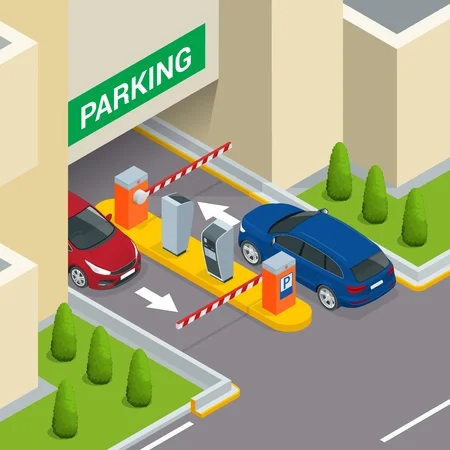
\includegraphics[height=06.2cm]{img/ch1-barrier-01.jpg}
	\caption{ Barrières d'entrée et de sortie}
  \label{ch1barrier}
\end{figure}

\textbf{1- Les barrières manuelles : } sont actionnées manuellement par un opérateur, qui contrôle l'accès des véhicules à l'entrée et à la sortie du parking en levant ou abaissant la barrière à l'aide d'une télécommande ou d'un levier. Les barrières manuelles sont souvent utilisées dans les petits parkings ou les parkings résidentiels où il y a un trafic relativement faible et où il n'est pas nécessaire de contrôler l'accès de manière automatique.

\textbf{2- Les barrières automatiques : } sont actionnées par un système électronique et sont équipées de capteurs de mouvement qui détectent la présence d'un véhicule. Lorsqu'un véhicule s'approche de la barrière, le système électronique déclenche l'ouverture ou la fermeture de la barrière pour permettre ou interdire l'accès. Les barrières automatiques sont souvent utilisées dans les parkings publics ou commerciaux où il y a un trafic plus important et où il est nécessaire de contrôler l'accès de manière efficace.

\subsubsection{ Les panneaux de signalisation}
Les panneaux de signalisation dans les parkings aident les conducteurs et les piétons à naviguer dans le parking en leur fournissant des informations sur la circulation, le stationnement et les règles de sécurité. Ils permettent est de faciliter la circulation et le stationnement des véhicules, de minimiser les risques d'accidents et de garantir la sécurité des piétons. Les panneaux doivent être clairs, visibles et conformes aux normes de signalisation routière en vigueur. Ils peuvent être fixes ou électroniques et être accompagnés d'autres dispositifs de contrôle de la circulation.
voici quelques panneaux dans l'image suivante \ref{ch1plak}

\begin{figure}[H]
	\centering
	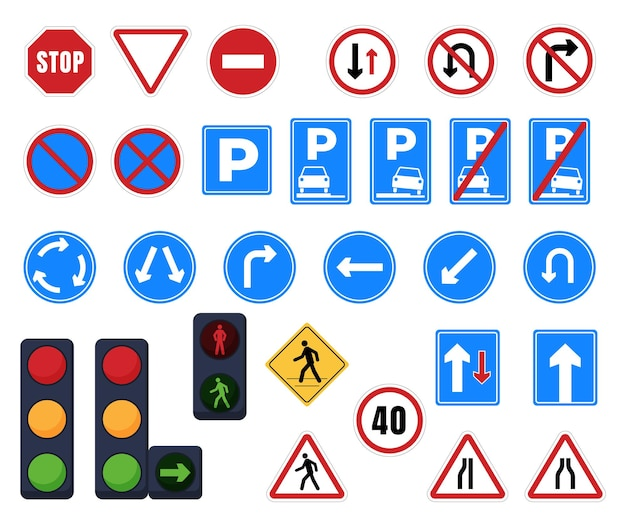
\includegraphics[height=06.5cm]{img/ch1-plak-01.jpg}
	\caption{Panneaux de signalisation}
 \label{ch1plak}
\end{figure}


\subsubsection{Les capteurs de stationnement}
Les capteurs utilisés dans les parkings sont des dispositifs électroniques qui sont conçus pour détecter la présence de véhicules dans une place de stationnement. Ces capteurs peuvent être installés dans les surfaces de stationnement, tels que les planchers ou les trottoirs, et peuvent être connectés à un système de gestion de parking pour surveiller l'occupation des places de stationnement en temps réel.

Les capteurs peuvent fonctionner de différentes manières, mais la plupart utilisent des technologies telles que les ultrasons, les champs magnétiques ou les capteurs de pression pour détecter la présence d'un véhicule. Certains capteurs peuvent également mesurer la durée de stationnement des véhicules et signaler tout dépassement de temps. l'image au dessous \ref{ch1sensor} illustre un des types de capteurs de rue 

\begin{figure}[H]
	\centering
	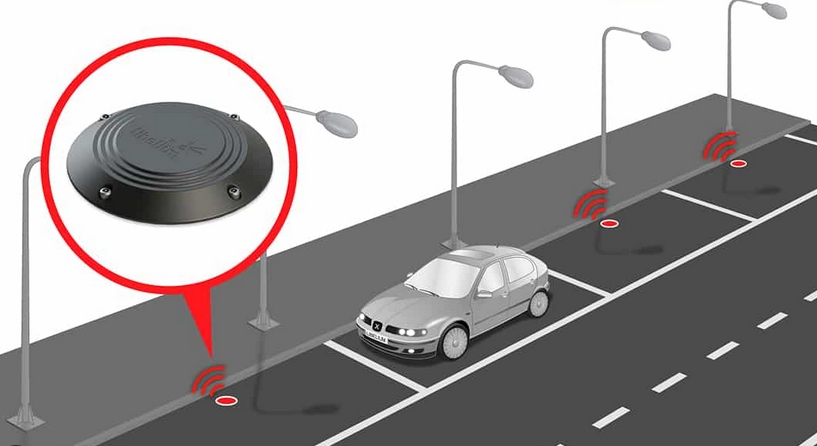
\includegraphics[height=05cm]{img/ch1-sensor-01.jpg}
	\caption{Les capteurs}
 \label{ch1sensor}
\end{figure}

% \subsubsection{ Les lecteurs de plaques d'immatriculation}

% Les lecteurs de plaques d'immatriculation, également appelés systèmes de reconnaissance automatique des plaques d'immatriculation comme montre la figure \ref{img}, sont des dispositifs utilisés dans les parkings pour capturer et reconnaître les plaques d'immatriculation des véhicules entrant et sortant. Ces lecteurs utilisent des caméras spéciales et des logiciels de reconnaissance optique des caractères pour analyser les images des plaques d'immatriculation et extraire les informations textuelles.

% L'objectif principal de ces systèmes est d'automatiser le processus d'identification des véhicules ce qui facilite par conséquent la traçabilité des véhicules dans le parking. Grâce à  cette automatisation, les erreurs humaines liées à la saisie manuelle des informations sont réduites.
% Les informations extraites des plaques d'immatriculation sont enregistrées dans le système de gestion du parking qui peut également enregistrer les données relatives aux véhicules entrants et sortants, telles que l'heure d'entrée et de sortie, la durée de stationnement, les transactions de paiement, etc. Ces données sont traités de manière sécurisée et conforme aux réglementations sur la protection des données personnelles. Des mesures appropriées doivent être prises pour garantir la sécurité et la confidentialité des données.

% \begin{figure}[H]
% 	\centering
% 	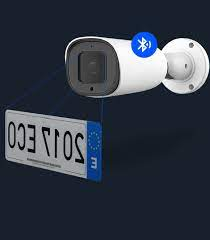
\includegraphics[height=05cm]{ch2-plate_read.jpg}
% 	\caption{Lecteurs de plaques d'immatriculation}
%  \label{img}
% \end{figure}

\subsubsection{Les bornes de paiement}
Les bornes de paiement \ref{img1} utilisées dans les parking sont des dispositifs électroniques autonomes qui offrent aux utilisateurs différentes options pour effectuer des paiements de manière automatisée (rapide, pratique et sécurisée) sans avoir besoin d'interagir avec un caissier ou un employé. En plus du paiement, ces bornes ont également la capacité d'émettre des tickets de paiement \cite{ch2_Transpor19}.

Lorsqu'un utilisateur souhaite payer son stationnement, il peut utiliser des cartes de bancaires, insérer des pièces de monnaie, des billets de banque ou utiliser des badges d'abonnement. Certaines bornes de paiement prennent également en charge les paiements mobiles, permettant aux utilisateurs de payer via des applications mobiles ou des portefeuilles électroniques. Ces options de paiement offrent aux utilisateurs une flexibilité lorsqu'ils règlent leurs frais de stationnement.
Une fois le paiement effectué, la borne génère un ticket de paiement qui sert de preuve de paiement et de validation du stationnement.

\begin{figure}[H]
	\centering
	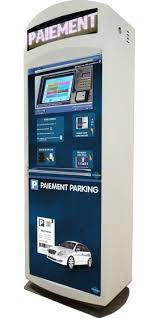
\includegraphics[height=07cm]{ch2-Bornes_pay.jpg}
	\caption{ Bornes de paiement}
 \label{img1}
\end{figure}

\section{Étude d'existant}

L'étude de l'existant en matière de systèmes de gestion de parking en Algérie révèle une diversité de solutions utilisées dans différents parkings à travers le pays. La plupart des parkings publics qu'on a visité utilisent des systèmes de gestion traditionnels basés sur des tickets papier ou des barrières manuelles gérées par le personnel.
On cite dans ce qui suit cinq exemples de parkings où ces méthodes sont en place :
\subsection{Parking Bézier - Tafourah - Alger}



Il s'agit d'un parking à plusieurs étages, public pour tous, et l'argent payé est calculé en fonction de la durée de stationnement

Lorsque vous arrivez à l'entrée du parking, vous trouverez un employé qui notera la plaque d'immatriculation du véhicule et l'heure d'entrée et vous remettra un ticket

Le ticket contient un table composé des heures de la journée de 6 h à 23 h

L'heure que vous avez entrée est cochée afin que vous sachiez à quelle heure vous avez entré

Vous recherchez un endroit pour garer la voiture et la garer

Et quand vous voulez quitter le parking, vous donnez ce ticket à un employé, et il calcule le temps approximatif que cela a pris et vous indique le prix.

Le prix le plus bas qui peut être payé est de 100 dinars si cela prend moins ou égal à 2 heures, et après les deux premières heures, 50 dinars seront ajoutés par heure. 
au dessous \ref{Bézier} une image réelle du parking Bézier qui se situe à Tafourah - wilaya d'Alger.

\begin{figure}
	\centering
	\includegraphics[height=07.5cm]{img/ch2-Parking Bézier - Tafourah - Alger.jpg}
	\caption{Parking Bézier - Tafourah - Alger}
 \label{Bézier}
\end{figure}

\subsection{Parking de l'université d'Alger1 - Ben Youssef Ben Khadda - Alger}  



C'est un parking pour les employés travaillant à l'université \ref{Khadda}, l'entrée est la même que la sortie, et il est géré par des personnes sans aucun outil technologique.

Lorsque le véhicule arrive à l'entrée du parking, le gardien vérifie son droit d'entrée en reconnaissant le conducteur du véhicule, ou le conducteur du véhicule voyant la carte de droit d'accès.

Si le gardien décide d'entrer dans le véhicule, il ouvre la porte, laisse entrer le véhicule et commence à chercher une place pour garer le véhicule.

L'un des plus gros problèmes dont souffre cette situation est que le propriétaire de la voiture ne sait pas s'il y a une place disponible pour garer sa voiture, et il peut devoir chercher et perdre du temps, puis quitter le parking pour chercher une place. Garez la voiture ailleurs.

\begin{figure}[H]
	\centering
	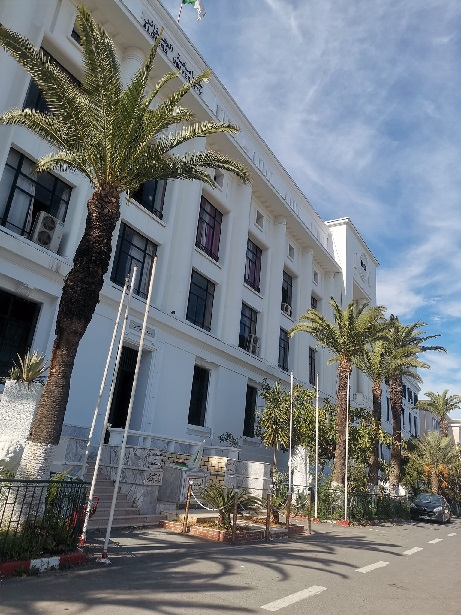
\includegraphics[height=07.5cm]{ch2-Parking de l'université centrale, Université Yusuf bin Khadda.jpg}
	\caption{Parking de l'université d'Alger1 - Ben Youssef Ben Khadda - Alger}
 \label{Khadda}
\end{figure}

% \subsection{ Parking avec ascenseur - centre d'Oran}
% Ce parking à plusieurs étages est équipé d'un ascenseur pour faciliter l'accès aux différents niveaux.
% À l'entrée du parking, un membre du personnel du parking remet un ticket manuscrit au propriétaire de la voiture. Ce dernier est alors invité à laisser les clés de sa voiture et à indiquer l'heure de retour prévue pour la récupérer.

\subsection{Parking Ali Mellah - premier mai - Alger}
C'est un parking semi-automatique où, quand le chauffeur arrive à l'entrée du parking, un agent vous extrait  un ticket apartir d'une machine, puis le client rentre et cherche un espace vide pour garer son voiture.
À la sortie le chauffeur donne le ticket à un autre agent afin de calculer le montant à payer.

\subsection{Parking de l'aéroport Houari Boumédiène - Alger}
Le parking en question est un parking en surface accessible au public \ref{Boumédiène}, et les frais de stationnement sont calculés en fonction de la durée de stationnement.
\\
Lorsqu'un véhicule arrive au parking, il se trouve face à une barrière fermée munie d'un bouton. En appuyant sur ce bouton, un ticket est généré, comprenant un QR-code ainsi que d'autres informations pertinentes. Par la suite, la barrière s'ouvre, permettant ainsi au véhicule d'accéder au parking.
\\
En ce qui concerne le paiement, une borne de paiement est mise à disposition pour effectuer le règlement en espèces, que ce soit sous forme de billets ou de pièces. De plus, la borne est en mesure de rendre la monnaie si nécessaire.
\\
Une fois le paiement effectué, il est important de sortir rapidement du parking en se dirigeant vers la sortie désignée. À la sortie, une barrière est présente et s'ouvre en scannant le QR-code présent sur le ticket.
\\
Dans le cas où le paiement n'a pas été effectué, il est nécessaire de se rendre à une sortie spécifique où un poste de garde est situé. A cette endroit, il sera possible de régler les frais de stationnement pour pouvoir quitter le parking.
\begin{figure}[H]
	\centering
	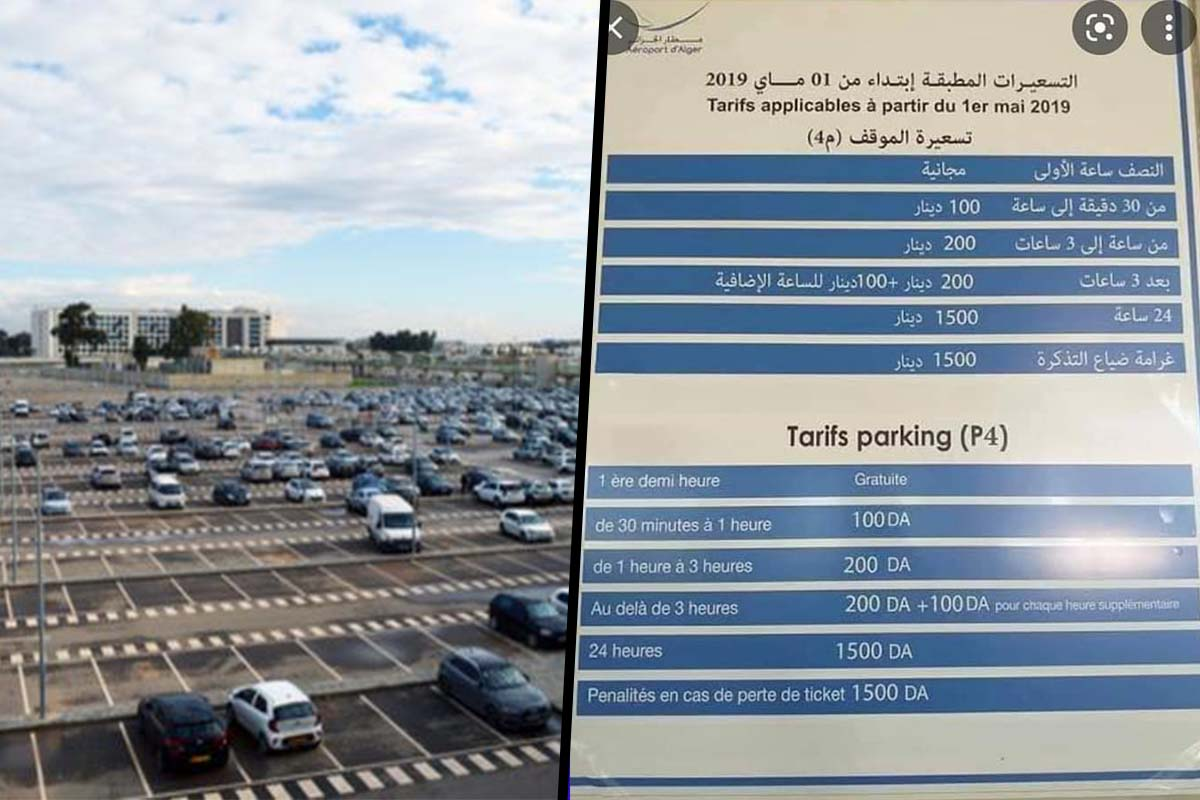
\includegraphics[height=08cm]{img/ch2-Parking aéroport à Alger Houari Boumédiène Airport.jpg}
	\caption{Parking de l'aéroport Houari Boumédiène}
 \label{Boumédiène}
\end{figure}
L'aéroport adopte une technologie de paiement électronique pour les cartes de stationnement, selon laquelle le propriétaire de la voiture doit payer la valeur du billet en fonction des heures d'attente dans un dispositif électronique qui lui donne une carte de dégagement de manière automatique, lui permettant de sortir automatiquement de la porte.

  
\textbf{L'étude réalisée met en évidence les lacunes suivantes dans les systèmes de gestion de parking :}
\begin{enumerate}
   \item [$\bullet$] Congestion à l'entrée et à la sortie du parking : Les barrières manuelles ou les méthodes de paiement traditionnelles peuvent entraîner des files d'attente importantes, ce qui provoque des embouteillages aux heures de pointe.
   \item [$\bullet$] Difficulté à trouver une place de stationnement : En raison de l'absence de visibilité sur les places disponibles, les conducteurs peuvent perdre du temps à chercher une place pour garer leur voiture, ce qui entraîne des retards et de la frustration.
   \item [$\bullet$] Manque d'information sur la disponibilité des places : Les conducteurs n'ont pas d'indications en temps réel sur la disponibilité des places de stationnement, ce qui les oblige à entrer dans le parking sans savoir s'il y a des espaces vacants.
   \item [$\bullet$] Stationnement désorganisé : En l'absence d'un système de guidage efficace, les voitures sont souvent garées de manière aléatoire à l'intérieur du parking, ce qui rend difficile la recherche d'une place disponible.
   \item [$\bullet$] Risque de perte du billet de stationnement : Si un conducteur perd son billet de stationnement, il peut être confronté à des frais supplémentaires ou à des difficultés pour sortir du parking.
   \item [$\bullet$] Manque de sécurité : Les systèmes de gestion actuels nécessitent souvent de laisser les clés de la voiture au personnel du parking, ce qui peut créer des risques de vol ou d'utilisation non autorisée du véhicule.
\end{enumerate}
Ces lacunes soulignent la nécessité d'améliorer les systèmes de gestion de parking en utilisant des technologies avancées. Ces solutions permettraient d'optimiser l'utilisation de l'espace de stationnement, de réduire les embouteillages, d'améliorer la sécurité et de faciliter l'expérience des conducteurs.

\section{Conclusion}

Dans le premier chapitre, nous avons abordé les divers aspects des parkings, notamment les différents types de parkings, la gestion des parkings et les systèmes de gestion des parkings. Nous avons présenté également les outils utilisés dans un système de gestion des parkings et procédé à une étude de l'existant pour mieux cerner les problèmes auxquels sont confrontés les parkings étudiés.
Dans le chapitre deux, nous nous penchons sur l'apprentissage automatique et la vision par ordinateur.
%---------------------------------------------------------------
%-- https://en.wikipedia.org/wiki/Parking
%-- https://codedelaroute.io/blog/parking-public/
%-- https://www.yespark.fr/edito/lexique-parking/parking-public-prive-definition-reglementation
%-- https://les-fourrieres.fr/guides-actualites/parking-prive-a-usage-public-quelles-sont-les-regles/
%-- https://parking-gery.com/9095_Quelle-est-la-difference-entre-un-parking-public-et-un-parking-prive-.html
%-- 
%-- 
%-- 
%-- 

